\documentclass[12pt]{article}
%%%%%%%%%%%%%%%%%%%%%%%%%%%%%
% Preambulo

%Paquetes para el formato en español (símblos de ñ, acentos ...)
\usepackage[T1]{fontenc}
\usepackage[utf8]{inputenc}
\usepackage[spanish,es-tabla]{babel}
%Paquete para modificar tamaño de sangria
\parindent=0cm  
%Paquete para expresiones matemáticas
\usepackage{amsmath}
\usepackage{amssymb,amsfonts,latexsym,cancel}
%Paquete para colocar gráficas
\usepackage{graphicx}
%Paquete para convertir figuras de formato eps a pdf
\usepackage{epstopdf}
%Paquete para gráficas y tablas (para indicar donde colocar la tabla o figura)
\usepackage{float}
%Paquete para colocar varias figuras dentro del entorno figura
\usepackage{subfigure}
%Paquete para dar formato a las tablas
\usepackage{array}
\usepackage{longtable}
%Paquete para colocar un nuevo entorno para las tablas y que cada colomna quede con formato matemático
\newcolumntype{E}{>{$}c<{$}}
%Paquete para la restricción de matrices
\setcounter{MaxMatrixCols}{40}
%Paquete para texto en negrita para expresiones matemáticas
\usepackage{bm}

%CONFIGURACIÓN DE MÁRGENES, ENCABEZADO Y LA PARTE INFERIOR

%%%%%%%%%%%%%%%%%%%%%%%%%%%%%%%%%%%%%%
%% Paquetes o configuración nueva. 
%---->%%%%%%%%%%%%%%%%%%%%%%%%%%%%%%%%
\usepackage[lmargin=2cm,rmargin=2cm,top=2.5cm,
bottom=2cm]{geometry} %Paquete para tamaño de márgenes izquierdo, derecho, altura y ancho
\usepackage{fancyhdr} %Paquete para comenzar a dar un formato al documento
\pagestyle{fancy} %Comando para dar estilo al paquete fancyhdr
\fancyhead{} %Paquete para eleminamos definiciones previas en la parte superior
\fancyhead[C]{Desigualdad socioeconómica y pobreza en el distrito Chuschi, periodo 2000-2019} %Comando para dar información en la parte superior, la C indica en la parte CENTRAL.
\fancyhead[R]{
\includegraphics[scale=0.03]{figuras/Logo}}%Comando para dar imagen en la parte superior, la R indica en la parte DERECHA.
\fancyfoot{}
\fancyfoot[R]{\thepage} %Comando para colcar el numero de pagina en la parte INFERIOR DERECHA
\fancyfoot[L]{Edison Achalma} %Paquete para colcar el numero de pagina en la parte INFERIOR IZQUIERDA
\renewcommand{\headrulewidth}{0.9pt} %Comando para la línea de la parte superior
\renewcommand{\footrulewidth}{0.5pt} %Comando para la línea de la parte inferior, si no queremos las líneas ponemos 0pt
%---->%%%%%%%%%%%%%%%%%%%%%%%%%%%%%%%%


\begin{document}

%TÍTULO O PORTADA

\begin{titlepage}
\begin{center} %Información centrada
\vspace*{2\baselineskip} %Comando para dar un epacio, al comienzo de la pagina se pone un *
\hrule height 3pt %Comando para la línea horizontal de la parte supeior
\vspace*{0.5\baselineskip} %despues de la lína genera un epacio de o.5pt
{\Huge \textbf{Universidad Nacional San Cristóbal de Huamanga}}\\[0.1cm] %Huge es para el tamaño de letra
{\large \textbf{ESCUELA PROFESIONAL DE ECONOMÍA}}
\vspace*{0.5\baselineskip}
\hrule %Comando para la línea horizontal de la parte inferior
\vspace*{7\baselineskip}


\includegraphics[scale=0.15]{figuras/cuadro}
\vspace*{2\baselineskip}

\textbf{ÁLGEBRA, CÁLCULO DIFERENCIAL \\
ejemplos y aplicaciones}

\vfill %Rellena espacio hasta el texto de la parte final 

ELMER EDISON ACHALMA MENDOZA \\
\today
\end{center}
\end{titlepage}

%TABLA DE CONTENIDO

\renewcommand{\contentsname}{Contenido} %Para CAMBIAR Índice con Contenido, si no queremos que aparesca solo dejamos en blanco la parte donde dice Contenido.
\tableofcontents
\thispagestyle{empty} %Quita el formato del articulo en la tabla de contenidos
\newpage %Para que el tabla de contenidos este en una nueva página

\setcounter{page}{1} %Para la enumeracion comience depues de tabla de contenidos

\section{Introducción}
En esta sección iniciamos con la introducción
\cite{Nombre1} \cite{Nombre2}

\section{Bases}
En esta sección mostramos las bases para los siguientes temas

\subsection{Productos notables}
\textbf{Cuadrado de un binomio:} \quad Sea
\[
(a+b)^{2} = (a+b)(a+b)
\]
En donde $a$ y $b$ representan números algebraicos cualesquiera, positivos o negativos. \\
Por tanto:

\[
(a+b)^{2} = a^{2} + 2ab + b^{2}
\]
Este resultado se puede expresar así: \\
El cuadrado de un binomio es igual al cuadrado del primer término, más el doble producto de los dos términos, mas el cuadrado del segundo. \\ [0.3cm] 
\textbf{Producto de dos binomios conjugados:} \\
Sea multiplicar $(a+b)$ por $(a-b)$, binomios que solo difieren por el signo del segundo término y que se llaman binomios conjugados. \\
Por tanto:
\[
(a+b)(a+b) = a^{2} - b^{2}
\]
El producto de los dos binomios conjugados s igual al cuadrado de el primer término menos el cuadrado de segundo término. \\ [0.3cm]
\textbf{Cuno de un binomio:} \\
Sea el binomio $(a+b)$, donde $a$ y $b$ representan términos algebraicos cualesquiera, positivos o negativos. Sea \\
\[
(a+b)^{3} = (a+b)(a+b)(a+b)
\]
Por tanto \\
El cubo de un binomio es igual al cubo del primer término, mas el tiple producto del primero por el segundo, mas el tripe producto del primero por el cuadrado del segundo, más el cubo de segundo.

\section{Cálculo diferencial}
El concepto que marca la diferencia entre el cálculo y el álgera y la trigonometría, es el límite. El límite es fundamental para determinar la tangente a una curva o la velocidad a un objeto.

\subsection{Razón de cambio y límites}
La velocidad promedio que tiene un cuerpo en movimiento durante un intervalo de tiempo, como la tabla \eqref{tabla1} se encuentra al dividir la distancia recorrida entre el lapso de tiempo. La unidad de medida es longitud por unidad de tiempo: kilómetros por otra que sea adecuada para el problema en cuestión.

\begin{table}[!ht]
\centering
\begin{tabular}{|c|c|c|}
\hline
elemento uno & elemento dos & elemento 3 \\
\hline
elemento uno & elemento dos & elemento 3 \\
\hline
elemento uno & elemento dos & elemento 3 \\
\hline
\end{tabular}
\caption{Usando el entorno normal}
\label{tabla1}
\end{table}

\subsection{Límites laterales y límites al infinito}
Para que una función $f$ tenga límite $L$ cuando $x$ se aproxima a $c$, debe estar definidas a ambos lados de $c$, y los valores de $f(x)$ deben aproximarse a $L$ a medida que $x$ se aproxima a $c$. Debido a ello, los límites ordinarios se llaman bilaterales.

Aun cuando $f$ no tenga un límite bilateral en $c$, podría tener un límite lateral, esto es, un límite si la aproximación  es solo por un lado. Si la aproximación es por la derecha, el límite es un lateral derecho. Si es por la izquierda, es un límite lateral izquierdo. Como en la figura \eqref{figura1}

\begin{figure}[H]
\centering
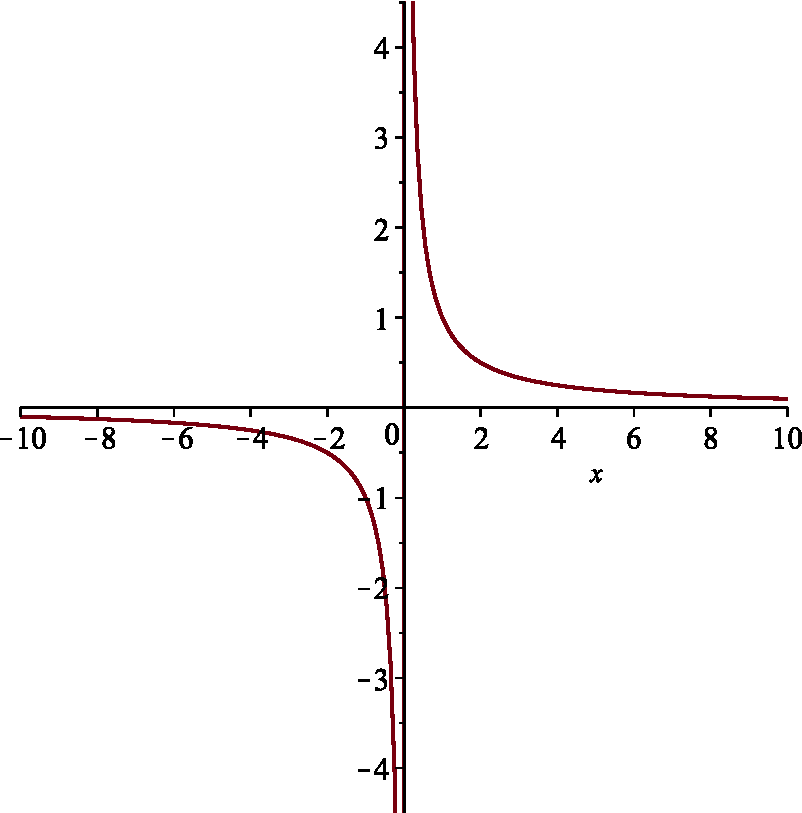
\includegraphics[scale=0.4]{figuras/grafica}
\caption{Gráfica de $y=1/x$}
\label{figura1}
\end{figure}

\subsection{Continuidad}
Cuando se dibujan los valores de una función, ya sea generados en un laboratorio o recopilados en el campo, es frecuente que los puntos se unan mediante una curva continua para mostrar los valores de la función en los tiempos que no se midieron. \\
Al hacerlo, suponemos que estamos trabajando con una función continua, de manera que los resultados varían de forma continua de acuerdo con los datos, el lugar de saltar de un valor a otro sin tomar en cuenta los valores intermedios. El límite de una función continua cuando $x$ se aproxima a $c$ puede encontrarse solo calcular el valor de la función en $c$.
\cite{Nombre3}

Ahora colocamos una tabla con algunos valores

\begin{table}[H]
\centering
\begin{tabular}{|E|E|E|}
\hline
X & (X+1)^{2} & (X+1)^{3} \\ 
\hline
X & (X+1)^{2} & (X+1)^{3} \\ 
\hline
X & (X+1)^{2} & (X+1)^{3} \\ 
\hline
\end{tabular}
\caption{Usando el entorno matemático definido}
\label{tabla2}
\end{table}

Cuando se dibujan los valores de una función, ya sea generados en un laboratorio o recopilados en el campo, es frecuente que los puntos se unan mediante una curva continua para mostrar los valores de la función en los tiempos que no se midieron. \\
Al hacerlo, suponemos que estamos trabajando con una función continua, de manera que los resultados varían de forma continua de acuerdo con los datos, el lugar de saltar de un valor a otro sin tomar en cuenta los valores intermedios. El límite de una función continua cuando $x$ se aproxima a $c$ puede encontrarse solo calcular el valor de la función en $c$.
\cite{Nombre4}

\newpage
%\renewcommand{\refname}{Bibliografía} %Para CAMBIAR Referencias con Bibliografía, si no queremos que aparescasolo dejamos en blanco la parte donde dice Bibliofrafía.
\begin{thebibliography}{99} % 99 indica la cantidad máxima de referencias por colocar
\bibitem{Nombre1} Articulo o Libro 1, Autor 1, Año de referencia 1. 
\bibitem{Nombre2} Articulo o Libro 2, Autor 2, Año de referencia 2. 
\bibitem{Nombre3} Articulo o Libro 3, Autor 3, Año de referencia 3. 
\bibitem{Nombre4} Articulo o Libro 4, Autor 4, Año de referencia 4. 
\end{thebibliography}

\end{document}